\documentclass[12pt]{article}
\usepackage[margin=0.75in]{geometry}
\usepackage{graphicx}
\usepackage{multicol}
\usepackage{float}
\usepackage{upgreek}

% for dots in TOC:
\usepackage{tocloft}
\renewcommand{\cftsecleader}{\cftdotfill{\cftdotsep}}

\setlength{\parindent}{0mm}

\begin{document}

{\centering
\LARGE Physics I-II Lab Manual \par
}
\hfill \break

{\centering
\large Preface \par
}
\hfill \break \vspace{-4mm}

This is the lab manual for Physics 2211L, 2212L, 1111L, and 1112L taught by Dr. Nathan Harrison.
In some labs you will have to copy and paste small amounts of code;
it is recommended that you copy from the the original \LaTeX \ source, \textit{not} from the PDF file which often leads to formatting errors.
Another common mistake is to not unzip the Java-based simulations;
if the simulation opens but the screen is blank it is because you didn't unzip the file.
\vfill
\textcopyright \ Nathan Harrison 2018
\pagebreak \clearpage

\tableofcontents
\pagebreak \clearpage

\section{Surface area, volume, and density with uncertainty}

You will be studying the properties of 3 objects - a rectangular prism, a sphere, and a (partially) hollow cylinder.
Don’t forget to use the appropriate number of significant figures, units, and error bars.
When taking a measurement, use half of the smallest reading on the instrument as the error bar;
for example, for a ruler with mm markings, the error bar should be 0.5 mm.
Use the ``$\pm$'' symbol to report the error bar; for example, Width = $3.55 \pm 0.05$ cm.
\begin{enumerate}
\item Determine the mass of each object by using the electronic balance in the front of the room and record the results.
\item Determine the relevant dimensions of each object, measure them with the calipers, and record the results. 
\item Use your measurements to calculate the surface area, volume, and density of each object. Remember to propagate the error and report the error bar.
\item Use available resources to identify the material of the object. Site your source(s).
\end{enumerate}

\pagebreak \clearpage

\section{Constant acceleration 1-D motion and data fitting}

\underline{\textbf{Part 1}} \par
Suppose you throw a ball straight up with initial height 1.0 m and initial velocity 2.1 m/s.
Create a plot of the ball's height as a function of time (assume $t_{initial} = 0$).
\hfill \break
\hfill \break
Example of how to plot in SageMath:
\begin{verbatim}
t = var("t")
p1 = plot(sin(10*t) + sin(10.1*t), (t, 15, 40), color="red")
g = Graphics()
g += p1
g.show()
\end{verbatim}
\hfill \break \vspace{-4mm}

\underline{\textbf{Part 2}} \par
Sketch a plot of the ball's position on the $y_1$ axis as a function of time.
Repeat for the $y_2$ axis.
\begin{figure}[H]
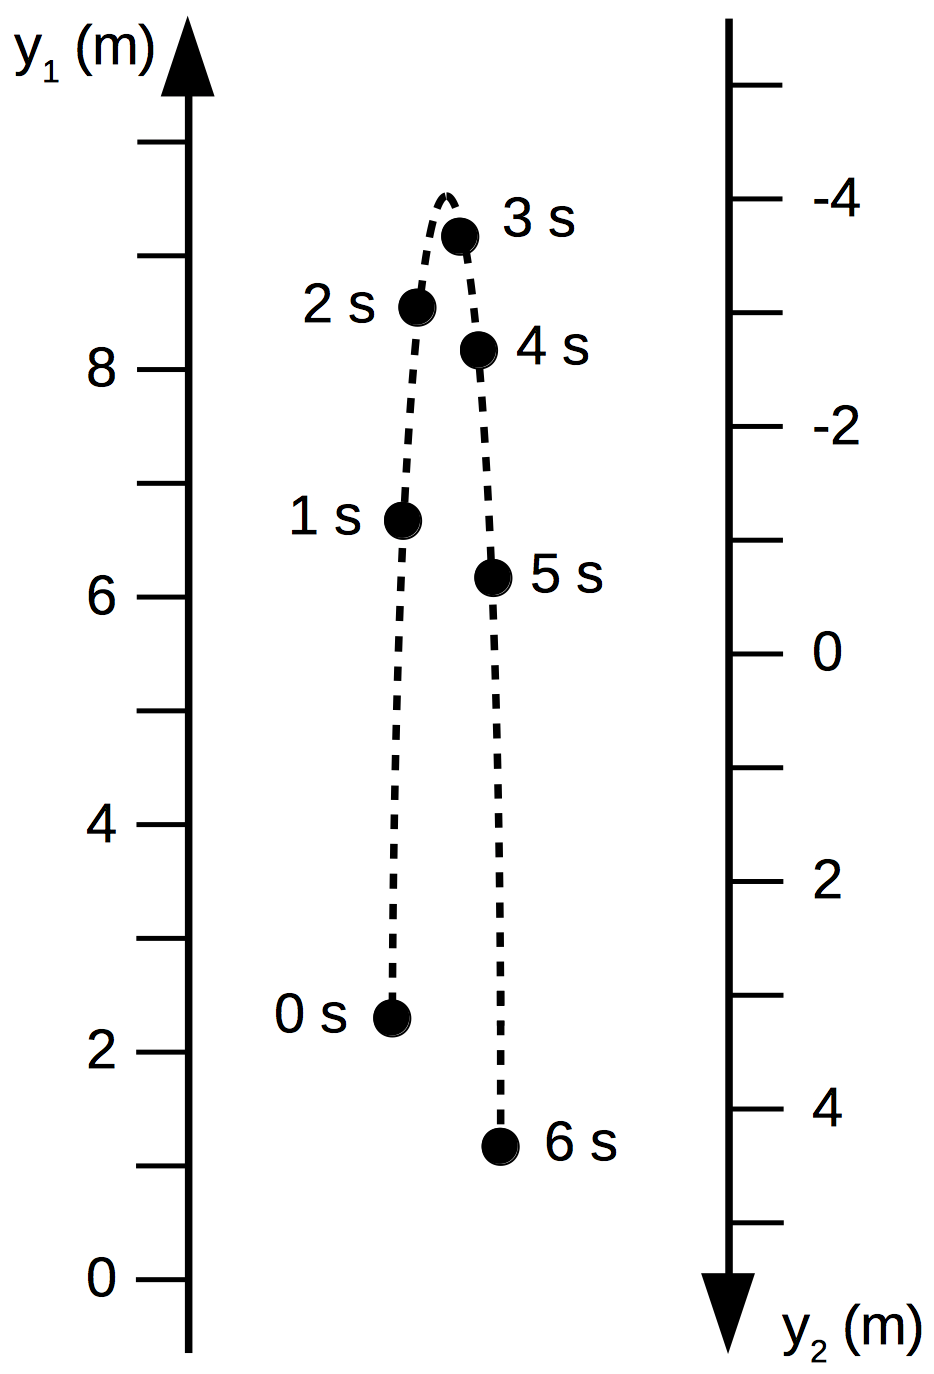
\includegraphics[scale=0.4]{figures/fitting1Dmotion/twoAxisFreeFall.png}
\end{figure}

\underline{\textbf{Part 3}} \par
Match each set of parameters below to one of the colored curves.
Briefly justify your answers.
\begin{itemize}
  \item $x_i = 0 \ m$, $v_i = -5 \ m/s$, $a = 5 \ m/s^2$
  \item $x_i = 0 \ m$, $v_i = 2 \ m/s$, $a = -4 \ m/s^2$
  \item $x_i = 8 \ m$, $v_i = 4 \ m/s$, $a = 3 \ m/s^2$
\end{itemize}
\begin{figure}[H]
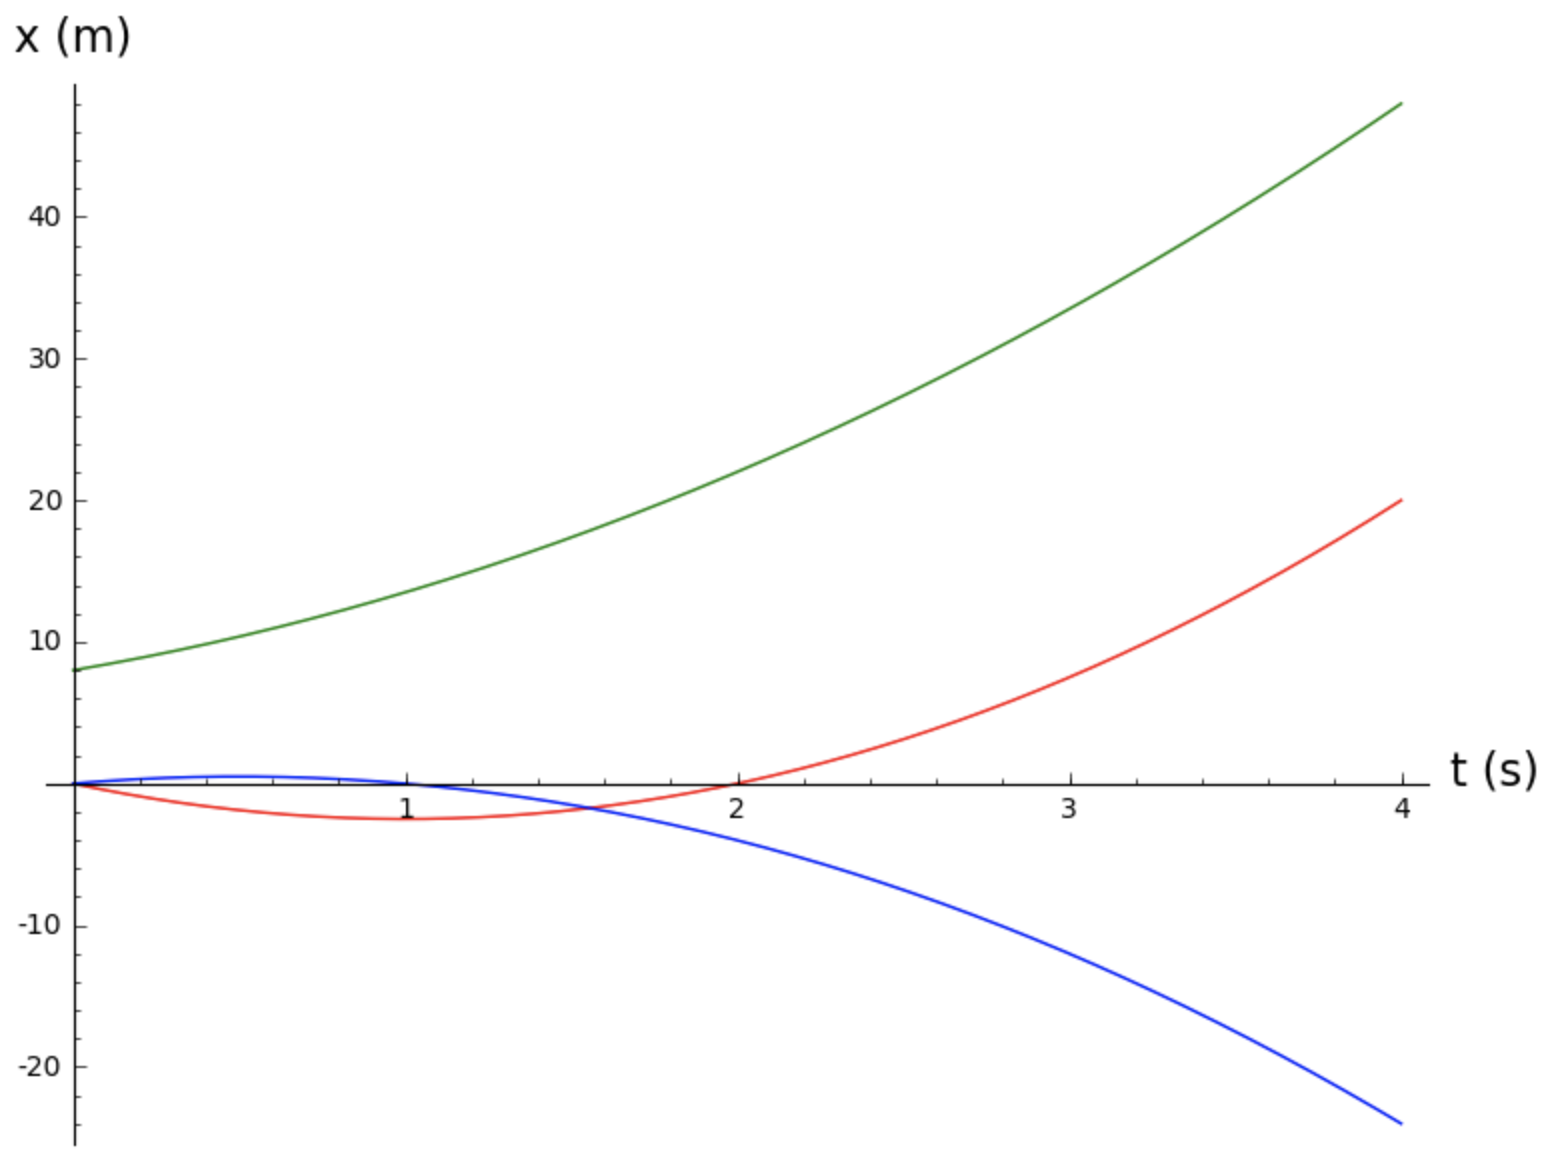
\includegraphics[scale=0.4]{figures/fitting1Dmotion/threeCurves.png}
\end{figure}

\underline{\textbf{Part 4}} \par
Now suppose you have some data collected from similar experiments on two other planets (different gravitational accelerations) (see Data section below).
Use this data to determine
(a) the gravitational acceleration of each planet,
(b) the orientation of the axis used in the experiment (up or down),
(c) the magnitude and direction (up or down) of the initial velocity, and
(d) the starting coordinate of the ball.
Use the following approach:
\begin{enumerate}
\item Download manfit-app.zip from https://github.com/naharrison/manual-fitter/releases, unzip it, and open the jar file.
\item From the unzipped folder, also open data/XYdata.txt and data/fitFunction.txt. Try to understand how the data in these files is being used by the application.
\item Copy the data below into XYdata.txt. Also modify fitFunction.txt to use a function that describes an object under constant acceleration: [0] + [1]*x + 0.5*[2]*x\string^2; the lines under the function are the minimum and maximum possible values for each parameter.
\item Restart the application and tune the parameters to determine the initial position, initial velocity, and acceleration.
\end{enumerate}

\pagebreak

\underline{\textbf{Data}} \par
\begin{multicols}{2}
\begin{verbatim}
Planet 1:
time (s)  y1 (m)
0.00      20.20
0.10      18.90
0.20      17.72
0.30      16.28
0.40      15.44
0.50      14.78
0.60      13.63
0.70      12.65
0.80      12.31
0.90      11.66
1.00      11.41
1.10      10.77
1.20      10.13
1.30      9.82
1.40      9.59
1.50      9.50
1.60      9.75
1.70      9.76
1.80      9.53
1.90      9.68
2.00      9.77
2.10      10.34
2.20      10.50
2.30      11.19
2.40      11.60
2.50      12.10
\end{verbatim}

\columnbreak

\begin{verbatim}
Planet 2:
time (s)  y2 (m)
0.00      -15.35
0.10      -14.17
0.20      -13.23
0.30      -12.16
0.40      -11.25
0.50      -10.41
0.60      -9.37
0.70      -7.82
0.80      -5.67
0.90      -3.65
1.00      -2.49
1.10      0.09
1.20      2.12
1.30      6.17
1.40      8.58
1.50      9.04
1.60      11.96
1.70      15.47
1.80      17.06
1.90      19.96
2.00      23.01
2.10      26.00
2.20      30.62
2.30      32.30
2.40      34.93
2.50      40.45
\end{verbatim}
\end{multicols}

\pagebreak \clearpage

\section{Projectile Motion}

In this lab you will be using the Interactive Physics (IP) software to simulate various kinds of two-dimensional motion and comparing the results to calculations.
Note that you can work from home through your web browser by going to my.ung.edu $\rightarrow$ Remote Access $\rightarrow$ Virtual Lab $\rightarrow$ Download Client $\rightarrow$ HTML 5 Browser $\rightarrow$ VMware Horizon HTML Access and logging in.
As always, do not copy exactly the examples given in these instructions.
Note that it may be possible to use the “guess and check” method in this lab to get approximately correct results; do not do this!
You must show all of your calculations.

Setup:
\begin{enumerate}
\item Open IP
\item Click View $\rightarrow$ Workspace and check ``Grid Lines'' and ``X,Y Axes''
\item Pan the screen so the origin is near the bottom left
\end{enumerate}

\underline{\textbf{Part 1}} \par
\begin{itemize}
\item Use the rectangle tool to create a floor and anchor it.
\item Use the circle tool to create a small circle, drag it to some height above the floor, and give it some velocity in the y-direction (right click the circle to adjust its values); keep $v_x = 0$ for now.
\item Create a second circle at a different height.
Calculate the necessary initial y-velocity so the two circles hit the floor at the same time.
Give the second circle this initial y-velocity.
\item Use the Windows ``Snipping Tool'' to take a screen shot of your initial conditions. (see fig.~\ref{fig:fig1})
\item Select both circles and click Windows $\rightarrow$ Appearance and check ``Track outline''.
Note: additional tracking settings are under World.
Run the simulation until both circles hit the floor.
Take another screenshot to show that your calculations were correct. (see fig.~\ref{fig:fig2})
\item Restart the simulation (clear the tracks by clicking World $\rightarrow$ Erase Track).
Give the circles some random (but reasonable) x-velocity to show they still hit the floor at the same time.
Run the simulation and take another screenshot. (see fig.~\ref{fig:fig3})
\end{itemize}
%
\begin{figure}[H]
\centering
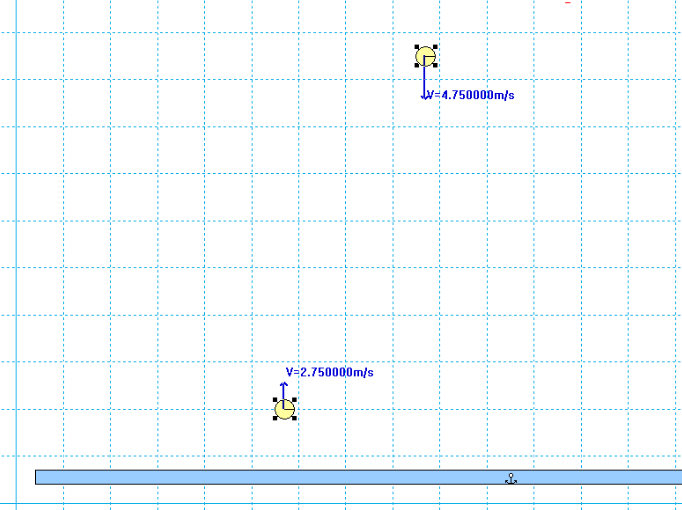
\includegraphics[scale=0.35]{figures/projectileMotion/fig1.png}
\caption{Initial conditions.}
\label{fig:fig1}
\end{figure}
%
\begin{figure}[H]
\centering
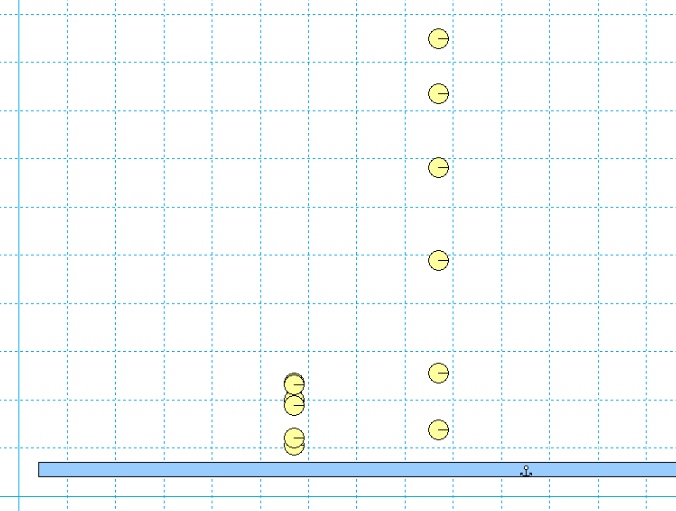
\includegraphics[scale=0.35]{figures/projectileMotion/fig2.png}
\caption{1-D motion.}
\label{fig:fig2}
\end{figure}
%
\begin{figure}[H]
\centering
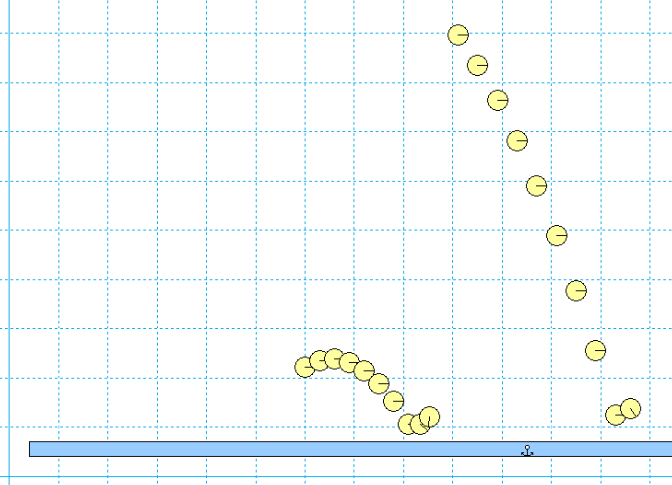
\includegraphics[scale=0.35]{figures/projectileMotion/fig3.png}
\caption{Projectile motion.}
\label{fig:fig3}
\end{figure}

\underline{\textbf{Part 2}} \par
\begin{itemize}
\item Using similar techniques as in Part 1, design an experiment where a projectile collides with a freely falling object.
Show relevant screen shots. (see figures~\ref{fig:fig2_1}~and~\ref{fig:fig2_2})
\end{itemize}
%
\begin{figure}[H]
\centering
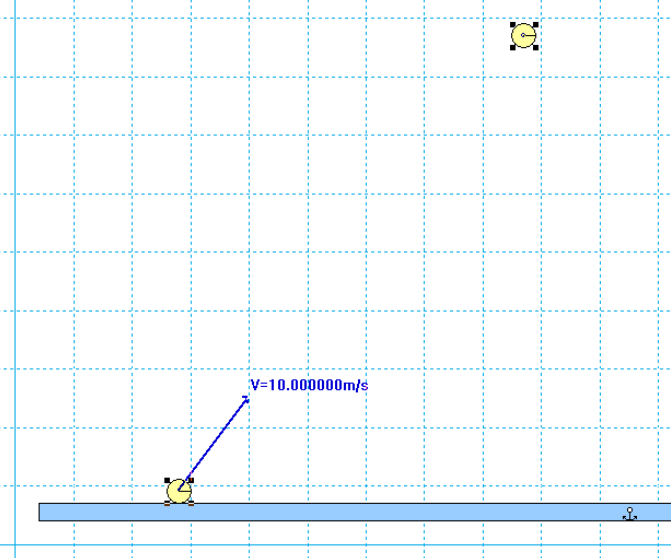
\includegraphics[scale=0.35]{figures/projectileMotion/fig2_1.png}
\caption{Part 2 initial conditions.}
\label{fig:fig2_1}
\end{figure}
%
\begin{figure}[H]
\centering
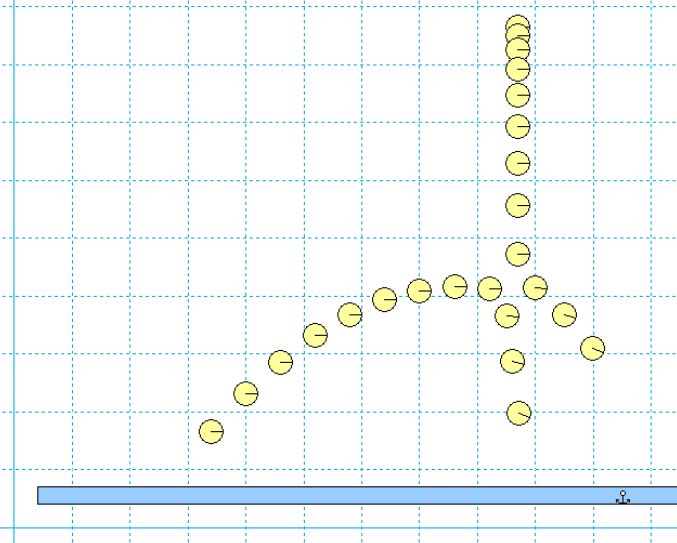
\includegraphics[scale=0.35]{figures/projectileMotion/fig2_2.png}
\caption{Part 2 result.}
\label{fig:fig2_2}
\end{figure}

\pagebreak \clearpage

\section{Forces}

In this lab you will investigate several applications of Newton's second law by calculating expected outcomes and comparing to (simulated) experiments.

Some comments:
\begin{enumerate}
\item When doing calculations, you treat objects like points, so in your simulations you should make your objects relatively small to achieve better results.
\item Each object in I.P. has coefficients of friction under its properties. When two objects are in contact, I.P. calculates the friction based on the smaller of the two values.
\item A stopwatch feature is available in I.P. under Measure $\rightarrow$ Time.
\end{enumerate}

\underline{\textbf{Part 1}} \par
For each diagram below, use a ruler to accurately draw the x and y components of the given vector.
Also use a ruler and protractor to measure the magnitudes $v$, $v_x$, and $v_y$, and at least one relevant angle.
Also write down the sign (positive or negative) of each component.
Confirm your measurements using the Pythagorean Theorem and trigonometry functions.
%
\begin{figure}[H]
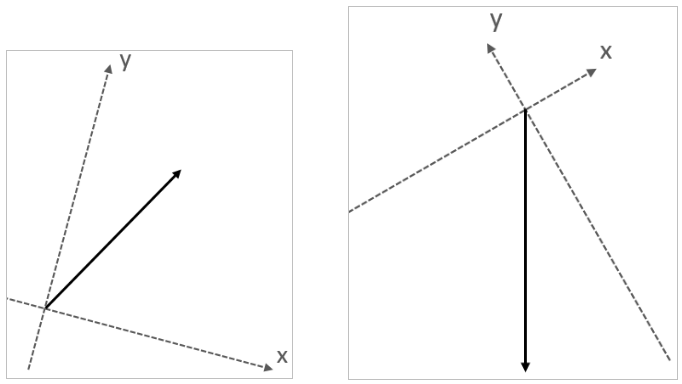
\includegraphics[scale=0.70]{figures/forces/fig1.png}
\end{figure}

\underline{\textbf{Part 2}} \par
Create an inclined ramp experiment.
Choose reasonable values for the angle of incline and the coefficients of friction (should be non-zero but small enough that the block slides). 
%
\begin{figure}[H]
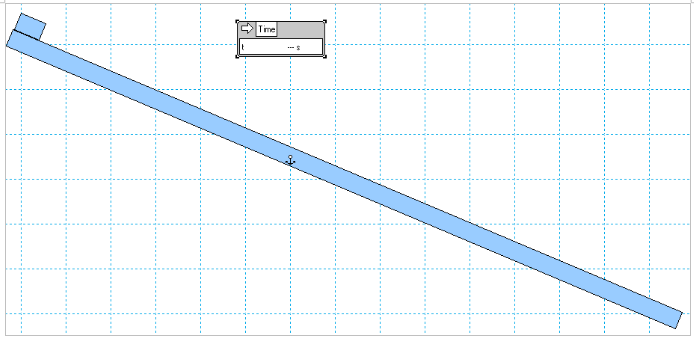
\includegraphics[scale=0.70]{figures/forces/fig2a.png}
\end{figure}
%
Calculate how long the block should take to travel some distance along the ramp.
Run your experiment and compare results.
Make sure to turn tracking on and to record relevant information and screenshots.
%
\begin{figure}[H]
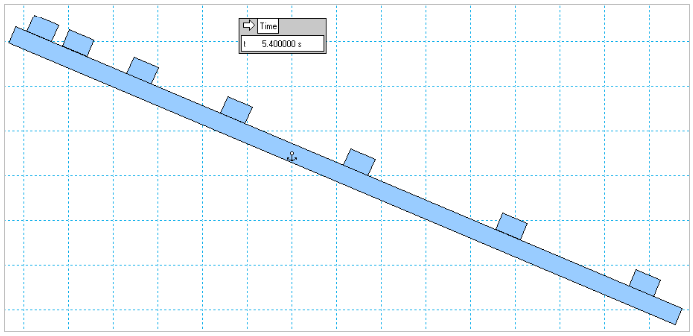
\includegraphics[scale=0.70]{figures/forces/fig2b.png}
\end{figure}

\underline{\textbf{Part 3}} \par
Create the experiment shown below.
Let the bottom block be $m_1$ and the top block be $m_2$.
The floor is a frictionless surface, however, some friction exists between $m_1$ and $m_2$.
A constant horizontal force, $F$, is applied to $m_1$.
If the force is small, then the friction between the two blocks keeps them together; but if the force is large enough, then block 1 slides out from underneath block 2.
Play around with some settings to get a feel for this.
Next, choose some reasonable values for $m_1$, $m_2$, and $F$.
Calculate the coefficient of static friction such that the blocks are right on the brink of slipping, and set this value in the experiment.
Run the experiment several times, changing slightly a few values to confirm that you found the correct coefficient of friction.

Note: here we are not very interested in the coefficient of kinetic friction, but to avoid bugs in IP make sure it is equal to the coefficient of static friction.
%
\begin{figure}[H]
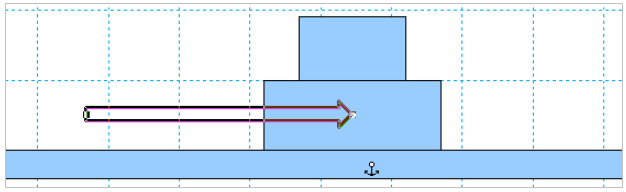
\includegraphics[scale=0.70]{figures/forces/fig3.png}
\end{figure}

\pagebreak \clearpage

\section{Energy}

In this lab you will explore how different forms of energy govern the dynamics of a given system.

Use Interactive Physics to set up the following experiment:
%
\begin{figure}[H]
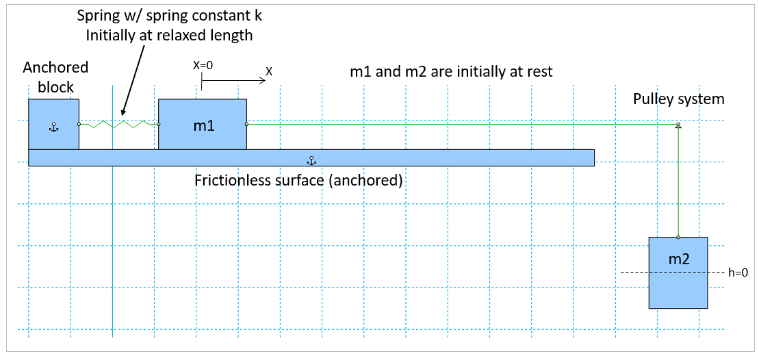
\includegraphics[scale=0.70]{figures/energy/fig1.png}
\end{figure}
%
Note that the diagram shows a suggested coordinate system choice, but you can define your own if you prefer.
Choose some random but reasonable values for k, m1, and m2 and run the simulation and observe the results.
Before proceeding, discuss with your lab partners why you think the systems behaves the way it does (you don't need to be too quantitative yet).

\bigskip

\underline{\textbf{Part 1}} \par
Determine the theoretical maximum displacement of m1 with respect to its initial position.
Use the simulation to confirm your result.

\bigskip

\underline{\textbf{Part 2}} \par
In terms of k, m1, m2, x, v, and g, use energy conservation to write down a general equation relating these quantities at any arbitrary time t.
Choose a random value of t and use IP to find the relevant quantities at this time.
Plug these values into your equation.
Is the equation (approximately) satisfied?

\pagebreak \clearpage

\section{Work and Power}

\underline{\textbf{Part 1}} \par
Use a constant horizontal force to push a block ($v_i = 0$) up a ramp that has friction.
Choose and record all relevant values.
Identify all forces present, label each one as conservative or non-conservative, and calculate the amount of work each one does on the block.
Use these work values to calculate the expected final velocity after some time interval.
Compare this calculation to the final velocity measured by IP.

\begin{figure}[H]
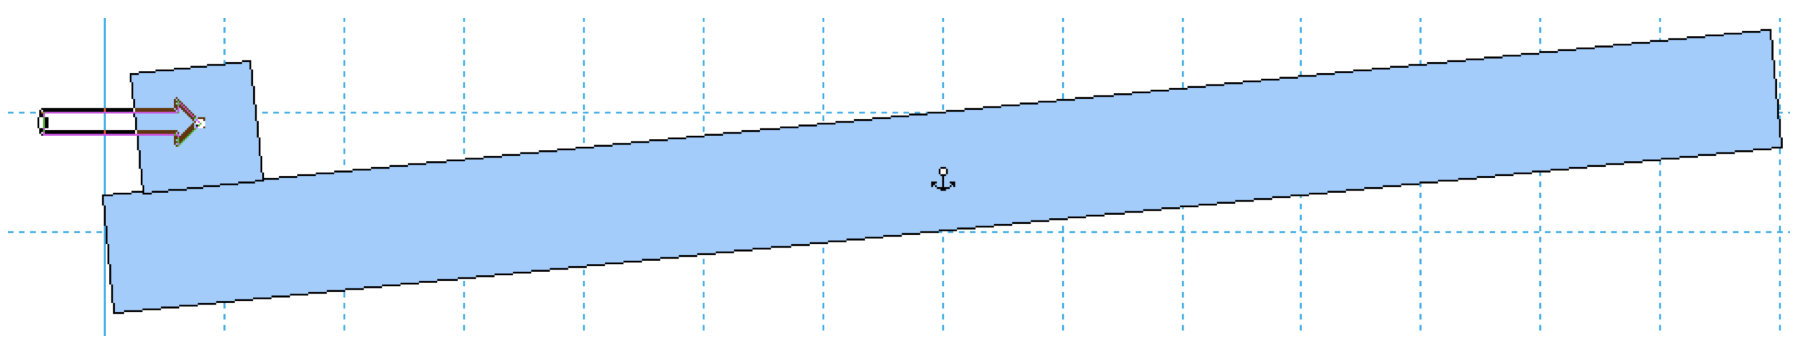
\includegraphics[scale=0.50]{figures/workPower/fig1.png}
\end{figure}


\underline{\textbf{Part 2}} \par
In this lab you will conduct a real life experiment to calculate your (or a lab mate's) maximum power output, with an uncertainty.

\begin{enumerate}
\item Write down your weight (with uncertainty) and convert to mass (in kg).
\item Gather relevant supplies (a ruler, stopwatch/smartphone, paper, pencil, and calculator) and go as a class to the staircase next to the Nesbitt building.
\item Use your ruler to measure the height of one stair. Also count the number of stairs to get the total elevation change from the bottom to the top. Make sure to propagate the error.
\item Have one person control the stop watch while another person runs up the hill next to the staircase as fast as possible. Record the time taken, with uncertainty. The runner and timer should coordinate a strategy so that the runner's velocity at the bottom is approximately equal to the velocity at the top; that way the change in energy is only due to the change in height. Include your strategy in your lab report. Although your stopwatch probably has very good precision, you may want to assign a larger time uncertainty due to the human error of starting and stopping at the right time.
\item Write down the relevant equations from class and calculate your power with uncertainty. Give your answer both in W and hp.
\end{enumerate}

\pagebreak \clearpage

\section{Momentum}

Suppose you are standing on a frictionless sled ($M_{you+sled} = 100$ kg) moving at 0.5 m/s.
You also have 22 blocks of mass 12 kg (i.e. $M_{total} = M_{you+sled}$ + 22(12 kg)).
You can boost your velocity by throwing the blocks horizontally at velocity 11 m/s in the opposite direction of your motion.
Create the following two plots: velocity vs the number of blocks thrown, and momentum vs the number of blocks thrown.
\hfill \break

Run the following simulation to test your results:
\begin{itemize}
\item Make sure you have Java JDK 1.8 installed
\item Download rocket-app.zip from https://github.com/naharrison/discrete-rocket/releases
\item Unzip the file and open rocket.jar
\item Click the green button to throw a block
\end{itemize}

\pagebreak \clearpage

\section{Torque}

\begin{verbatim}
https://phet.colorado.edu/sims/html/balancing-act/latest/balancing-act_en.html
Click "Game"
Complete all 4 levels - take screenshots of your results
\end{verbatim}

\pagebreak \clearpage

\section{Angular Kinematics}

In this lab you will explore the relationships between mass distributions, torques, angular momentum, and angular kinematics.
\hfill \break

Open Interactive Physics, turn gravity off, and create a T-shaped rotational object as shown.
Keep the thickness reasonably small.
You will have to attach the object to an anchor using a ``pin joint'' and attach the two parts of the T together with ``rigid joints.''
%
\begin{figure}[H]
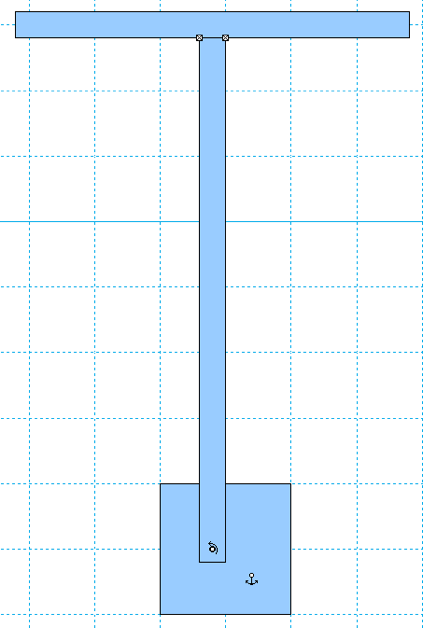
\includegraphics[scale=0.70]{figures/angularKinematics/figure1.png}
\end{figure}
%

\underline{\textbf{Part 1}} \par
Calculate the moment of inertia of the object about the base of the T.
Use the torque tool to apply a torque to the base of the T.
Measure the angular acceleration of the object for at least 4 values of torque.
Create a plot of $\alpha$ vs $\uptau$ and use this data to extract the object's moment of inertia.
Compare the result to your calculation.
\hfill \break

\underline{\textbf{Part 2}} \par
For a fixed value of torque, measure $\omega_i$ and $\omega_f$ over some time interval $\Delta t$.
Use this data to show that $\uptau = \Delta L / \Delta t$.
Repeat for a different value of torque.

\pagebreak \clearpage

\section{Orbits}

In this lab you will use SageMath to numerically calculate the paths for several different kinds of orbital motion.
\hfill \break

For simplicity, assume that for the given universe, planet, and unit system the product $GM_{planet} = 1$.
Also assume that the given satellite has a mass of 1.
Under these conditions the gravitational force is $F_g = 1/r^2$ and the requirement for circular motion is $F_c = v^2/r$.
(Do not make these assumptions outside of this lab.)
\hfill \break

\underline{\textbf{Part 0}} \par
Copy the orbit\_plot.sage script (below) and run the following example:
\begin{verbatim}
radius = var("radius")

blue_circle = circle((0, 0), 0.1, color="blue", fill=True, zorder=100, figsize=[5.5, 5.5])
planet_label = text("Planet", (0, 0), color="black", fontsize="large", zorder=101)

plot1 = orbit_plot(0.5, 0.0, 1.0, 1.0/(radius*radius), 0.01, 1.0, "green")
plot2 = orbit_plot(0.6, -1.0, 0.9, 1.0/(radius*radius), 0.01, 1.0, "red")

g = Graphics()
g += blue_circle
g += planet_label
g += plot1
g += plot2
g.set_axes_range(-0.8, 0.8, -0.8, 0.8)
g.show()
\end{verbatim}
%
\begin{figure}[H]
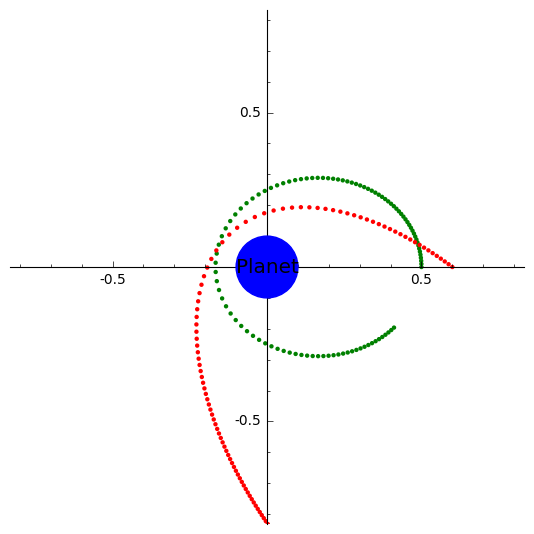
\includegraphics[scale=0.60]{figures/orbits/part0.png}
\end{figure}
%
Make sure you understand what each argument of orbit\_plot() means;
Refer to the table below:
\begin{enumerate}
  \item $x_i$ of the satellite ($y_i = 0$ by default)
  \item $v_{xi}$ of the satellite
  \item $v_{yi}$ of the satellite
  \item the gravitational force law, i.e. $F_g = 1/r^2$ (see above)
  \item the time interval between data points, make this smaller for more detail
  \item the path length at which the calculations stops, make this larger to see more of the path
  \item the color of the data points
\end{enumerate}
Adjust a few settings to see how they affect your resulting plot.
\hfill \break

\underline{\textbf{Part 1}} \par
Create two circular orbits of different radii.
Record your initial values and a screenshot of your plot.
%
\begin{figure}[H]
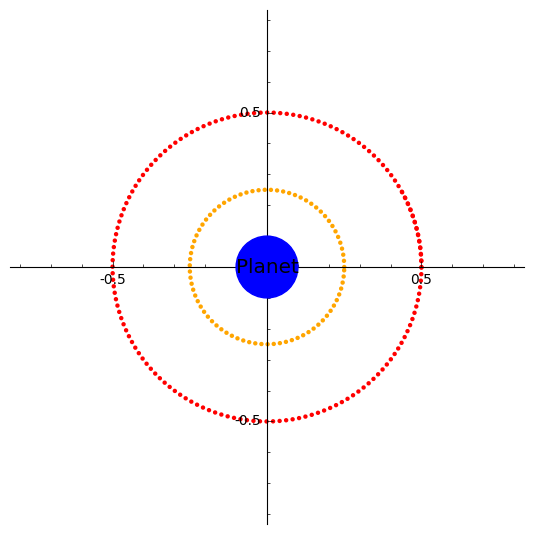
\includegraphics[scale=0.60]{figures/orbits/part1.png}
\end{figure}

\underline{\textbf{Part 2}} \par
a) Create an elliptical orbit by either
\begin{itemize}
\item making the velocity too large
\item making the velocity too small
\item making the velocity non-tangent to a circular path.
\end{itemize}
b) Create a case where the velocity is larger than the escape velocity.

Record your conditions and a screenshot of your plot.
%
\begin{figure}[H]
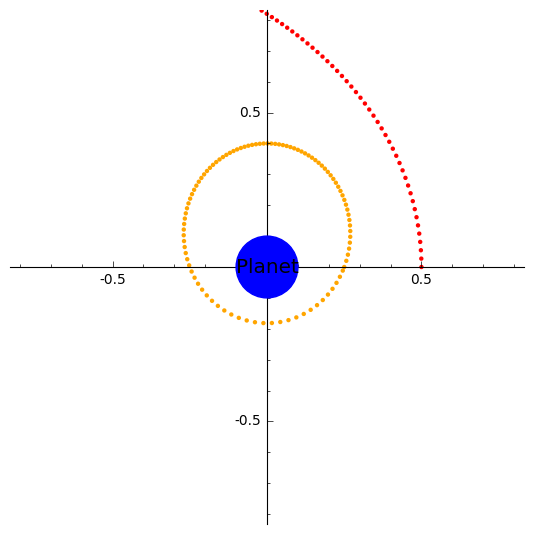
\includegraphics[scale=0.60]{figures/orbits/part2.png}
\end{figure}

\underline{\textbf{Part 3}} \par
Design your own universe with a different gravitational force law.
Experiment until you find an interesting result.
Record your conditions and a screenshot of your plot.
%
\begin{figure}[H]
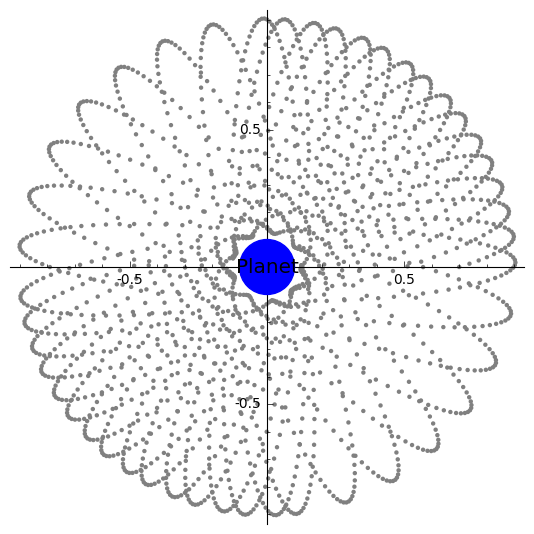
\includegraphics[scale=0.60]{figures/orbits/part3.png}
\end{figure}

\underline{orbit\_plot.sage} \par
\begin{verbatim}
__author__  = "Nathan Andrew Harrison"
__license__ = "GPL-3.0"

# see Goldstein & Poole 3.7 and 3.11
#                       ^^^     ^^^^
#                       2 second order ODEs converted to 4 1st order ODEs


def orbit_plot(radius_i, vx_i, vy_i, force, stepsize, endpt, plotcolor):

  # variables
  theta, thetaPrime, radius, radiusPrime, time = var("theta, thetaPrime, radius, radiusPrime, time")
  theta_i = 0.0
  
  # calculations
  x_i = radius_i*cos(theta_i)
  y_i = radius_i*sin(theta_i)
  radiusPrime_i = 2.0*x_i*vx_i + 2.0*y_i*vy_i
  thetaPrime_i = ((vy_i*x_i - y_i*vx_i)/(x_i*x_i))/(pow(y_i/x_i, 2.0) + 1.0)
  
  sol = desolve_system_rk4([thetaPrime, -2.0*radiusPrime*thetaPrime/radius, radiusPrime, -force + radius*thetaPrime*thetaPrime], [theta, thetaPrime, radius, radiusPrime], ics=[0, theta_i, thetaPrime_i, radius_i, radiusPrime_i], ivar=time, end_points=[0, endpt], step=stepsize)
  
  
  pts = [[m*cos(k), m*sin(k)] for j, k, l, m, n in sol]
  
  return list_plot(pts, color=plotcolor)
\end{verbatim}

\pagebreak \clearpage


\end{document}
